
\begin{figure}[h]
	\centering
	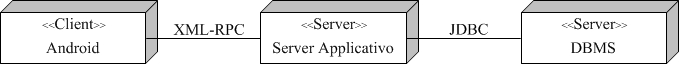
\includegraphics[width=0.7\textwidth]{Immagini/Architecture_Envisoring}
	\caption{Architecture Envisioning}
	\label{fig:ArchitectureEnvisoring}
\end{figure}
\noindent
In figura ~\ref{fig:Deployment Diagram} e ~\ref{fig:ArchitectureEnvisoring} sono mostrati il Deployment Diagram e l'Architecture Envisioning del sistema progettato per lo sviluppo dell’applicazione di Book Crossing. 

Si può osservare che si tratta di un’architettura \textbf{\textit{Three Tiers}}:
\begin{enumerate}
	\item A sinistra si individua il \textit{Client}, ovvero il dispositivo Android con il quale l'utente può interfacciarsi direttamente. Al suo interno si può osservare la presenza di un componente relativo all’interfaccia grafica e uno relativo alla gestione delle richieste per invio e ricezione di dati con il server;
	\item Nella parte centrale individuiamo gli altri due layer dell’architettura: server EC2 e Database Relazionale RDS. Il fatto di utilizzare Amazon Web Services (AWS) consente di avere questi due elementi integrati in un unico strato.
\end{enumerate}
\noindent
Per la comunicazione tra smartphone e EC2 utilizziamo un connettore basato su una socket TCP, mentre il server applicativo (EC2) si connette al DBMS (RDS Oracle) tramite il connettore OJDBC (Oracle Java DataBase Connectivity). 